\title{Video Analysis\\
1. \"Ubungsaufgabe}
\author{Philipp Omenitsch, xyzxyz\\
Marko Mlinaric, 0825603}
\date{\vspace{-5ex}}

\documentclass[]{scrartcl}

\usepackage{graphicx}
\usepackage{hyperref}
\usepackage{caption}
\usepackage{subcaption}

\begin{document}
\maketitle

\section{\"Uberblick zur Implementation und Source-Code}
Die 1. Aufgabe bestand darin ein Verfahren zur Segmentierung von Vordergrundobjekten in Videostreams zu implementieren. Daf\"ur haben wir zuerst den Versuch unternommen, die in der Angabe vorgestellte Methode \textbf{\textit{Color Mean and Variance}} zu implementieren. Als wir allerdings auf Probleme gesto\ss{}en sind, haben wir als Alternative die \textbf{\textit{ViBe}} Methode implementiert \cite{barnich2011vibe}.

Wir haben C++ und OpenCV gew\"ahlt um die Aufgabe zu l\"osen. Unser Source-Code besteht aus den beiden Files \texttt{main.h} und \texttt{main.cpp}.

In Header-File \texttt{main.h} befinden sich Deklarationen von Methoden und globale Variablen, die wir verwendet haben. Der Gro\ss{}teil der Implementation befindet sich im Sourcefile \texttt{main.cpp}. 



\section{Color Mean and Variance}\label{sec:cmv}
Bei der Color Mean and Variance Methode wird für jedes Pixel und jeden Farbkanal extra ein Modell gebaut. Jedes Pixel wird als eigenes Signal interpretiert, für das in der Initalisierungphase eine Normalverteilung mit $N(\mu, \sigma)$ gefunden wird. 

\paragraph{Adaptivit\"at} 
Um Veränderungen der externen Umst\"ande in das Modell einflie\ss{} zu lassen, flie\ss{} Hintergrund- und Vordergrundpixel, verschieden stark gewichtet wieder in das Modell mit ein.
\paragraph{Probleme} 
Bei CMV hatten wir vorallem das Problem, dass wenn Pixel nicht als Vordergrund erkannt werden, sie als Hintergrundpixel entsprechend stark gewichtet werden und unser Modell an entsprechenden Stellen sehr schnell eine hohe Varianz adaptiert, die mehr oder weniger fast alles als Hintergrund detektiert.

\section{ViBe}\label{sec:vibe}
ViBe ist ein Sample-basierter Algorithmus zur Segmentierung von Vordergrundobjekten in Videostreams. Das Hintergrundmodell besteht aus $width \times height \times nbSamples$ Samples, wobei $width$ und $height$ die Breite und H\"ohe des Videostreams bezeichnen und $nbSamples$ ein w\"ahlbarer Parameter f\"ur die Anzahl an Samples pro Pixel ist. 

\paragraph{Initalisierung}
F\"ur die Initialisierungedes Hintergrundmodells reicht ein einzelnes Frame, da f\"ur jedes Pixel auch aus der n\"aheren Umgebung gesamplet werden kann. In unserer Implementierung samplen wir dennoch aus mehreren Frames, da durch die Natur der Angabe davon auszugehen ist, dass es immer eine gewisse Anzahl an Initialisierungsframes geben wird und sich das positiv auf unser Modell auswirkt.

Segmentiert wird, indem der Wert jedes Pixels mit den entsprechenden Samples verglichen wird. Es wird gez\"ahlt f\"ur wie viele Samples, die Distanz kleiner einem festgelegten threshold ist. \"Uberschreiten diesen Wert mehr als \texttt{reqMatches} Pixel eines Samples, so wird angenommen, dass dieser Pixel zum Hintergrund geh\"ort.

\paragraph{Adaptivit\"at}
Sollte das Pixel Teil des Hintergrund sein, so wird das Hintergrundmodell zuf\"allig upgedatet. Im Schnitt jedes $n$-te Mal wird ein zuf\"alliges bestehendes Sample durch durch den Wert des aktuellen Pixel ersetzt. Ebenso wird jedes $n$-te Mal ein zuf\"alliges Sample eines zuf\"alligen Pixels in der Nachbarschaft durch den Wert des aktuellen Pixel ersetzt. Letzteres f\"uhrt dazu, dass der Hintergrund langsam in den Vordergrund \"uberl\"auft. $n$ wird im Code als \texttt{subsamplingFactor} bezeichnet.

\paragraph{Vergleich}
Wir haben durch diesen Algorithmus im Vergleich zu \textit{Color Mean and Variance} subjektiv deutlich sichtbare Verbesserungen erfahren. Um Rauschen noch etwas zu unterdr\"ucken und Komponenten deutlicher darzustellen, wenden wir f\"ur jedes segmentierte Bild noch \textit{Closing} an und f\"ullen Konturen, um L\"ocher in den segmentierten Objekten zu schließen, da wir annehmen, dass die Objekte in der Szene keine gro\ss{}en L\"ocher haben.

\begin{figure}[h!]
\centering
\begin{subfigure}{.5\textwidth}
  \centering
  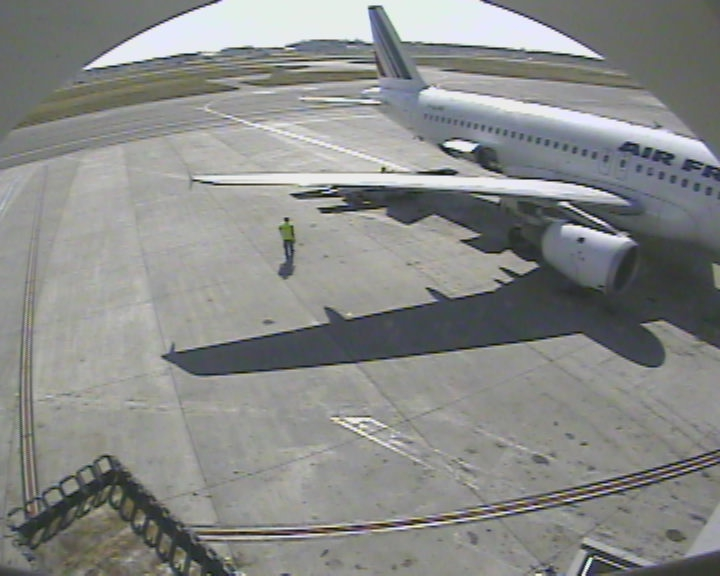
\includegraphics[width=.8\linewidth]{S3A3202_0100.jpeg}
  \caption{Originalbild}
  \label{fig:orig}
\end{subfigure}%
\begin{subfigure}{.5\textwidth}
  \centering
  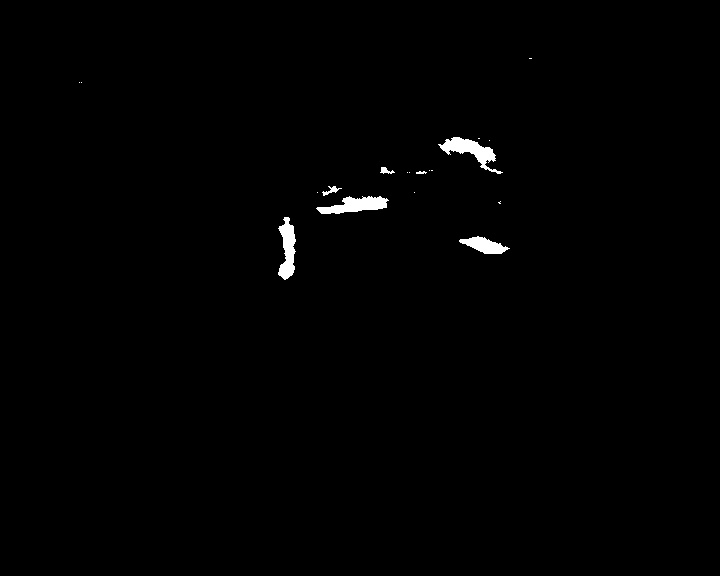
\includegraphics[width=.8\linewidth]{Seg_S3A3202_0100.jpeg}
  \caption{Segmentierung}
  \label{fig:seg}
\end{subfigure}
\caption{Vergleich Original und Segmentierung.}
\label{fig:vergleich}
\end{figure}

\begin{figure}[h!]
\centering
\begin{subfigure}{.5\textwidth}
  \centering
  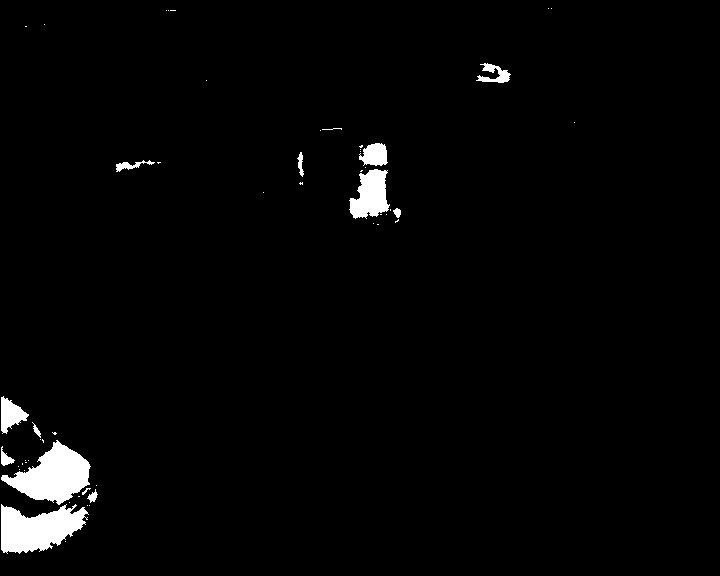
\includegraphics[width=.9\linewidth]{Seg_S36-A319-8_0175.jpeg}
  \caption{Segmentierung f\"ur Frame \#175}
  \label{fig:seg1}
\end{subfigure}%
\begin{subfigure}{.5\textwidth}
  \centering
  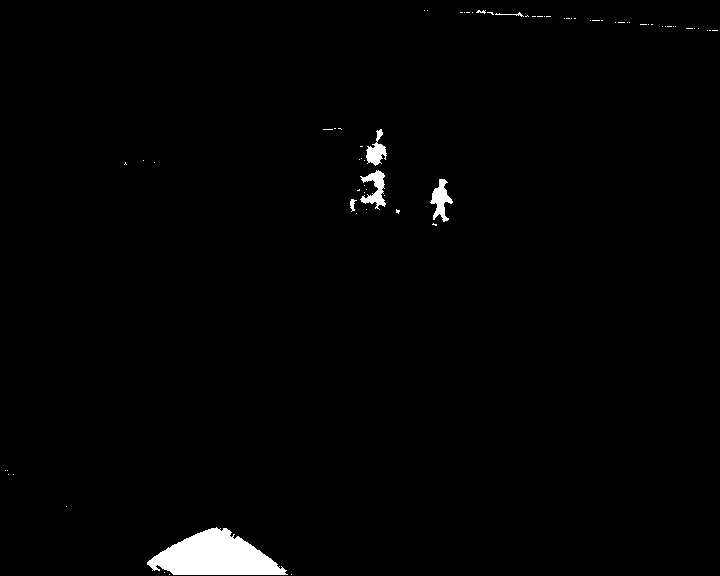
\includegraphics[width=.9\linewidth]{Seg_S36-A319-8_0222.jpeg}
  \caption{Segmentierung f\"ur Frame \#222}
  \label{fig:seg2}
\end{subfigure}
\begin{subfigure}{.5\textwidth}
  \centering
  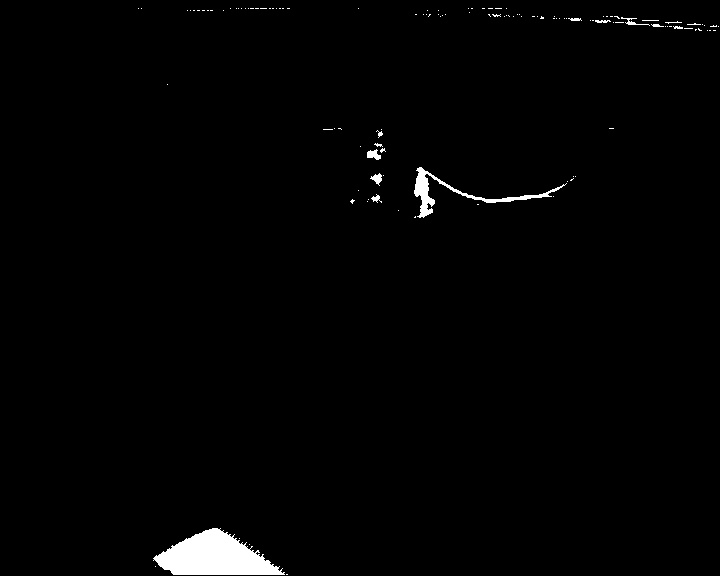
\includegraphics[width=.9\linewidth]{Seg_S36-A319-8_0264.jpeg}
  \caption{Segmentierung f\"ur Frame \#264}
  \label{fig:seg3}
\end{subfigure}%
\begin{subfigure}{.5\textwidth}
  \centering
  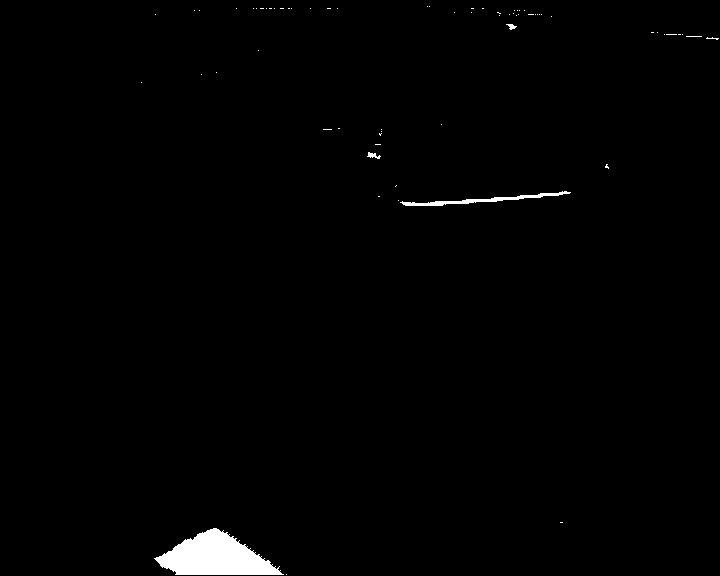
\includegraphics[width=.9\linewidth]{Seg_S36-A319-8_0316.jpeg}
  \caption{Segmentierung f\"ur Frame \#316}
  \label{fig:seg4}
\end{subfigure}
\begin{subfigure}{.5\textwidth}
  \centering
  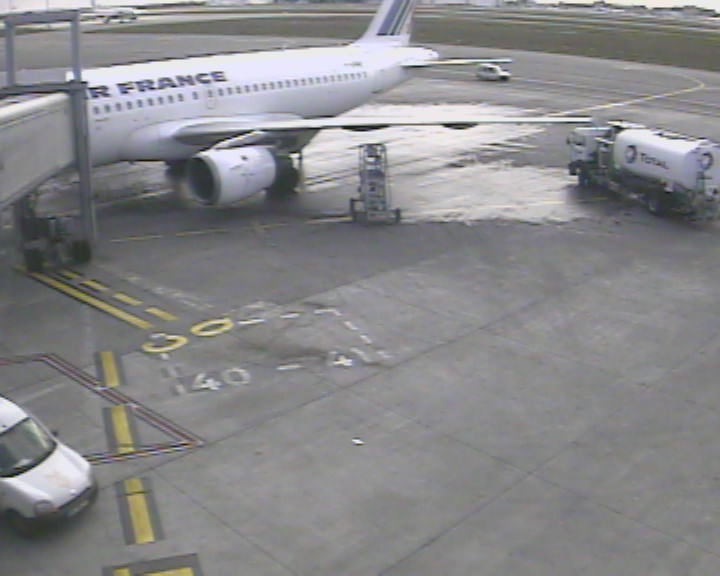
\includegraphics[width=.9\linewidth]{S36-A319-8_0175.jpeg}
  \caption{Original Frame \#175}
  \label{fig:orig1}
\end{subfigure}%
\begin{subfigure}{.5\textwidth}
  \centering
  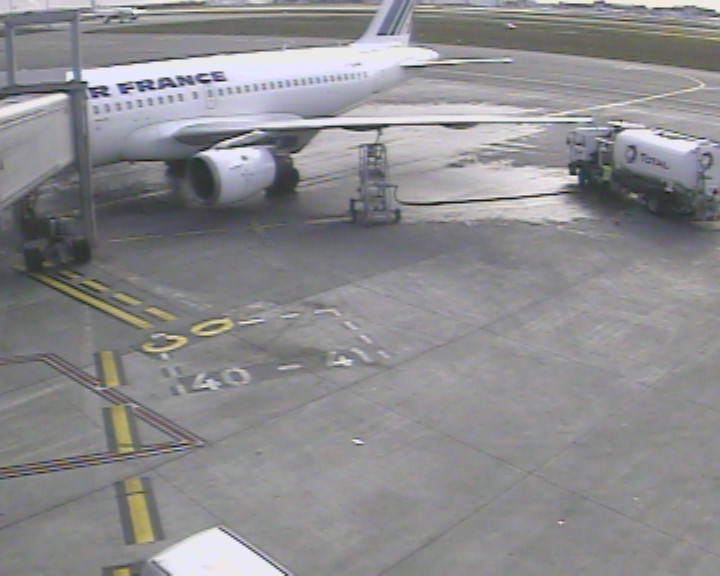
\includegraphics[width=.9\linewidth]{S36-A319-8_0316.jpeg}
  \caption{Original Frame \#316}
  \label{fig:orig2}
\end{subfigure}
\caption{Adaption. Objekt verschwindet in den Hintergrund.}
\label{fig:adaption}
\end{figure}


\bibliographystyle{ieeetr}
\bibliography{main}

\end{document}